\subsubsection{Generering af Map}
\noindent Map klassen generer et map til spillet. Denne består af en
simple liste af lister over, hvilket rooms hvert room er 
forbundet til.

Denne Process er kompliceret og kræver en uddybende forklaring. Problemet 
består i at afgøre hvordan man sikre at det samme map bliver genereret
hver gang spillet loades. 

\paragraph{Gem en map layout fil \\}
Denne løsning viste sig at være den bedste løsning for at sikre sig, at 
map layoutet kun skulle eksistere i en enkel folder i projektet.
Men det viste sig vanskelig at læse en sådan fil uafhængigt af pc'en 
programmet blev kørt på.

\paragraph{Lav en klasse som generer map layout filen \\}
Ultimativt blev dette løsningen, som benyttes i projektet. En MapCreator
klasse danner en map layout fil når dens konstruktor bliver kald.

En map klasse som store map layoutet kan nu læse layout filen og 
danne et map udfra denne fil.
Filen består af linjer med formen \textit{``leftRoomId, TopRoomId, RightRoomId, BottomRoomId''}. Den først linje dækker room 1, næste linje dækker room 2 osv.

Hver linje i map layout filen mappes til en liste af roomId'er,  der kan insertes i Map
klassens mapLayout listea. Denne Liste danner grundlaget for spillets map og 
diktere hvordan spilleren kan navigere i spillet. Denne mapping mellem strings og int array
er vist i \autoref{fig:RoomConverter}.

\begin{figure}[h]
  \centering
  \caption{viser illustrer hvordan en linje fra map layout filen omdannes til en liste af room id'er 
           som rummet er forbundet med. Dette er kerne mekanismen for hvordan en spiller kan navigere
           rund i spillet, da en spiller ikke kan bevæge sig fra et Room til et anden, der ikke er 
           i denne liste af forbindelser mellem det nuværende room og den ønskede bevægelses retning.}
  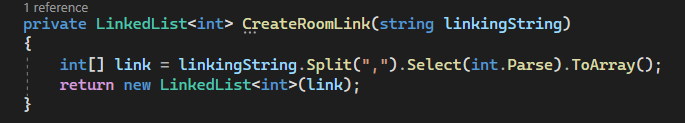
\includegraphics[scale=0.8]{02-Body/Implementering/GameEngineImplementering/Images/MappingRoomString.png}
  \label{fig:RoomConverter}
\end{figure}

\paragraph{Items og Enemies \\}
Som det sker for rooms, ligeledes sker der for enemies og items. MapCreator klassen
generer seperate filer for enemy positions og item lokationer. Map klassen 
kan herefter læse filen og mappe hver linje i filen til, en enemy eller item og 
placere det i det korrekte room.

